\begin{enumerate}[label=\thesection.\arabic*,ref=\thesection.\theenumi]
\item Write the five terms at n = 1, 2, 3, 4, 5 of the sequence and obtain the Z-transform of the series
\begin{align}
    x \brak{n} &=  -1, & n = 0 \\
    &=   \frac{x \brak{n-1}}{n}, & n > 0\\
    &=   0, & n < 0 
\end{align}

\solution

\iffalse
\let\negmedspace\undefined
\let\negthickspace\undefined
\documentclass[journal,12pt,twocolumn]{IEEEtran}
\usepackage{cite}
\usepackage{amsmath,amssymb,amsfonts}
\usepackage{graphicx}
\usepackage{textcomp}
\usepackage{xcolor}
\usepackage{txfonts}
\usepackage{listings}
\usepackage{enumitem}
\usepackage{mathtools}
\usepackage{gensymb}
\usepackage{comment}
\usepackage[breaklinks=true]{hyperref}
\usepackage{tkz-euclide} 
\usepackage{listings}
\usepackage{gvv}                                        
\def\inputGnumericTable{}                                 
\usepackage[latin1]{inputenc}                                
\usepackage{color}                                            
\usepackage{array}                                            
\usepackage{longtable}                                       
\usepackage{calc}                                             
\usepackage{multirow}                                         
\usepackage{hhline}                                           
\usepackage{ifthen}                                           
\usepackage{lscape}
\usepackage[export]{adjustbox}

\newtheorem{theorem}{Theorem}[section]
\newtheorem{problem}{Problem}
\newtheorem{proposition}{Proposition}[section]
\newtheorem{lemma}{Lemma}[section]
\newtheorem{corollary}[theorem]{Corollary}
\newtheorem{example}{Example}[section]
\newtheorem{definition}[problem]{Definition}
\newcommand{\BEQA}{\begin{eqnarray}}
\newcommand{\EEQA}{\end{eqnarray}}
\newcommand{\define}{\stackrel{\triangle}{=}}
\newtheorem{rem}{Remark}

\begin{document}
\parindent 0px
\bibliographystyle{IEEEtran}

\vspace{3cm}

\title{}
\author{EE23BTECH11217 - Prajwal M$^{*}$
}
\maketitle
\newpage
\bigskip

 \renewcommand{\thefigure}{\theenumi}
 \renewcommand{\thetable}{\theenumi}


\section*{Exercise 9.1}

\noindent \textbf{12} \hspace{2pt}Write the five terms at n = 1, 2, 3, 4, 5 of the sequence and obtain the Z-transform of the series
\begin{align}
    x \brak{n} &=  -1, & n = 0 \\
    &=   \frac{x \brak{n-1}}{n}, & n > 0\\
    &=   0, & n < 0 
\end{align}

\noindent Solution:
\fi
\noindent
\begin{align}
	x \brak{1} & = \frac{x \brak{0}}{1} = -1 \\
x \brak{2} & = \frac{x \brak{1}}{2} = -\frac{1}{2} \\
	x \brak{3} & = \frac{x \brak{2}}{3} = -\frac{1}{\brak{2} \brak{3}} = -\frac{1}{6}\\
	x \brak{4} & = \frac{x \brak{3}}{4} = -\frac{1}{\brak{2}   \brak{3} \brak{4}} = -\frac{1}{24}\\
	x \brak{5} & = \frac{x \brak{4}}{5} = -\frac{1}{\brak{2} \brak{3} \brak{4} \brak{5}} = -\frac{1}{120} \\
    x \brak{n} & = \frac{-1}{n!}  \brak{u \brak{n}} \label{x(n)}
\end{align}
\begin{align}
	x \brak{n} & \system{Z} X \brak{z} 
\end{align}

\begin{figure}[h]
   \centering
   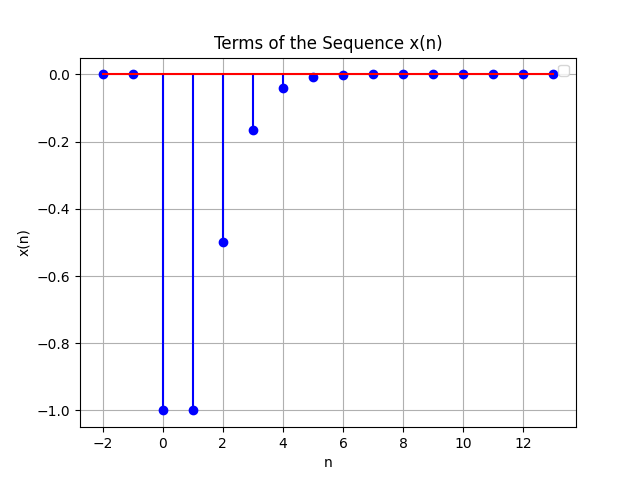
\includegraphics[width=1\columnwidth]{ncert-maths/11/9/1/12/figs/plot.png}
   \caption{Plot of x(n) vs n}
   \label{fig: 9.1.12.1}
\end{figure}

\begin{align}
    X \brak{z} & = \sum_{n=-\infty}^{\infty} x \brak{n}   z^{-n} \\
    \notag \text{using \eqref{x(n)}, } \\
    & = \sum_{n=-\infty}^{\infty} \frac{-1}{n!}  u \brak{n}   z^{-n} \\
    & = \sum_{n=0}^{\infty} \frac{-1}{n!}   z^{-n} \\
    & = - e^{z^{-1}} &  \cbrak{z\in\mathbb{C} : z \neq 0} 
\end{align}

\begin{table}[h]
    \centering
      \begin{tabular}{|c|c|c|}
    \hline
    	\textbf{Symbol} & \textbf{Value} & \textbf{Description} \\
    \hline
	  $x(n)$ & $\frac{-1}{n!}$ & general term of the series \\
    \hline
	  $X(z)$ & $- e^{z^{-1}}$ &Z-transform of x(n) \\
    \hline 
	  $u(n)$ & &unit step function \\
    \hline
  \end{tabular}

    \caption{Parameters}
    \label{tab: 9.1.12.1}
\end{table}


%\end{document}


\item Subba Rao started work in 1995 at an annual salary of Rs. 5000 and received an increment of Rs. 200 each year. In which year did his income reach Rs. 7000?

\solution

\iffalse
\let\negmedspace\undefined
\let\negthickspace\undefined
\documentclass[journal,12pt,twocolumn]{IEEEtran}
\usepackage{cite}
\usepackage{amsmath,amssymb,amsfonts,amsthm}
\usepackage{algorithmic}
\usepackage{graphicx}
\usepackage{textcomp}
\usepackage{xcolor}
\usepackage{txfonts}
\usepackage{listings}
\usepackage{enumitem}
\usepackage{mathtools}
\usepackage{gensymb}
\usepackage{comment}
\usepackage[breaklinks=true]{hyperref}
\usepackage{tkz-euclide}
\usepackage{listings}
\usepackage{gvv}
\def\inputGnumericTable{}
\usepackage[latin1]{inputenc}
\usepackage{color}
\usepackage{array}
\usepackage{longtable}
\usepackage{calc}
\usepackage{multirow}
\usepackage{hhline}
\usepackage{ifthen}
\usepackage{lscape}

\newtheorem{theorem}{Theorem}[section]
\newtheorem{problem}{Problem}
\newtheorem{proposition}{Proposition}[section]
\newtheorem{lemma}{Lemma}[section]
\newtheorem{corollary}[theorem]{Corollary}
\newtheorem{example}{Example}[section]
\newtheorem{definition}[problem]{Definition}
\newcommand{\BEQA}{\begin{eqnarray}}
\newcommand{\EEQA}{\end{eqnarray}}
\newcommand{\define}{\stackrel{\triangle}{=}}
\theoremstyle{remark}
\newtheorem{rem}{Remark}
\begin{document}

\bibliographystyle{IEEEtran}
\vspace{3cm}

\title{NCERT Discrete - 10.5.2.19}
\author{EE23BTECH11007 - Aneesh Kadiyala$^{*}$% <-this % stops a space
}
\maketitle
\newpage
\bigskip

\renewcommand{\thefigure}{\theenumi}
\renewcommand{\thetable}{\theenumi}
\vspace{3cm}
\textbf{Question 10.5.2.19:} Subba Rao started work in 1995 at an annual salary of Rs. 5000 and received an increment of Rs. 200 each year. In which year did his income reach Rs. 7000?

\solution
\fi
\begin{table}[h!]
    \centering
    \begin{tabular}{ | c | c | c | }
        \hline
        Parameter & Value & Description \\
        \hline
        $x(0)$ & 5000 & Initial Income \\
        \hline
        $d$ & 200 & Annual Increment (Common Difference) \\
        \hline
        $x(n)$ & $(x(0) + nd)u(n)$ & $n^{th}$ term of the AP \\
        \hline
    \end{tabular}
    \caption{Input Parameters}
    \label{tab:math_10_5_2_19}
\end{table}
From the values given in \tabref{tab:math_10_5_2_19}:
\begin{align}
7000 &= 5000 + 200n \\
\implies 2000 &= 200n \\
\therefore n &= 10
\end{align}
\begin{figure}[h!]
    \centering
    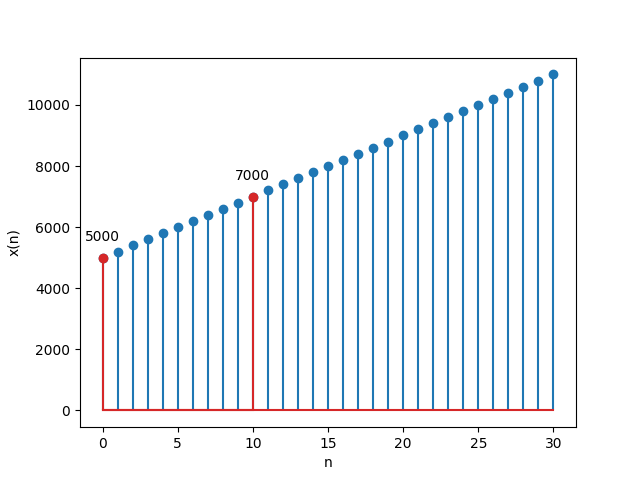
\includegraphics[width=\columnwidth]{ncert-maths/10/5/2/19/figs/10_5_2_19.png}
    \caption{Plot of $x(n)$ vs $n$. See \tabref{tab:math_10_5_2_19} for details.}
    \label{fig:math_10_5_2_19}
\end{figure}
Let Z-transform of $x(n)$ be $X(z)$.
\begin{align}
X(z) &= \frac{x(0)}{1 - z^{-1}} + \frac{dz^{-1}}{(1 - z^{-1})^2} \quad |z| > 1
\end{align}
Using the values from \tabref{tab:math_10_5_2_19}:
\begin{align}
X(z) &= \frac{5000}{1 - z^{-1}} + \frac{200z^{-1}}{(1 - z^{-1})^2} \quad |z| > 1
\end{align}
%\end{document}


\end{enumerate}
